In this section, we examine the effective frequency responses induced by translation via the regularized least-squares and hybrid interpolation filters as a function of source azimuth.
As described in \secref{sec:06_Simulation_Framework:Azimuth_Dependence}, for these simulations, we let $L_\text{in} = 4$, pick $\Delta = 0.5$~m and $s_0 = 2.5$~m (so $\gamma = 10$), and interpolate to $\vec{r}_0 = (0, 0, 0)$.
(Recall that these quantities are defined in \secref{sec:06_Simulation_Framework:Linear_Geometry} for a linear array geometry.)

The induced frequency responses are plotted in \figref{fig:08_Proposed_Method:Azimuth_Dependence}.
For the regularized least-squares interpolation filters (see \figref{fig:08_Proposed_Method:Azimuth_Dependence:Pinv}), we see that the frequency response is largely flat below a critical frequency (cf.~\citet[Fig.~4b]{TylkaChoueiri2016}), whereas above that frequency, the response exhibits significant broadband deviations (e.g., for $\varphi_0 = 75^\circ, 90^\circ$) as well as sporadic notches.
Based on well-established psychoacoustic findings, we can expect these distortions to be more audible (that is, either more likely to be audible or more significantly distorted) than the comb-filtering response of the weighted average method \citep{Bucklein1981,Kates1984,Brunner2007}.%
\footnote{In particular, \citet{Bucklein1981} showed that spectral peaks are more audible than notches of the same width and height, and that broadband spectral features are more audible than narrow ones.
Additionally, psychoacoustic studies have shown that comb-filter responses can be imperceptible if the time-delay between the primary and secondary signals is long enough and/or if their relative levels are different enough \citep{Kates1984,Brunner2007}.}

\begin{figure*}[t]
    	\centering
    	\begin{subfigure}[b]{0.49\textwidth}
        		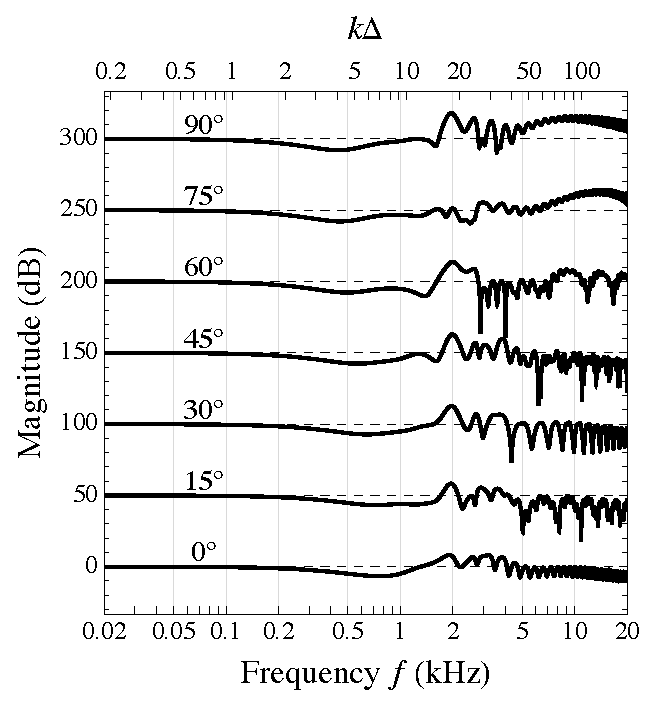
\includegraphics[width=\textwidth]{08_proposed_method/figures/sourceAz_freqResp_pinv.eps}
        		\caption{Regularized least-squares filters}
        		\label{fig:08_Proposed_Method:Azimuth_Dependence:Pinv}
    	\end{subfigure}
	\hfill
    	\begin{subfigure}[b]{0.49\textwidth}
        		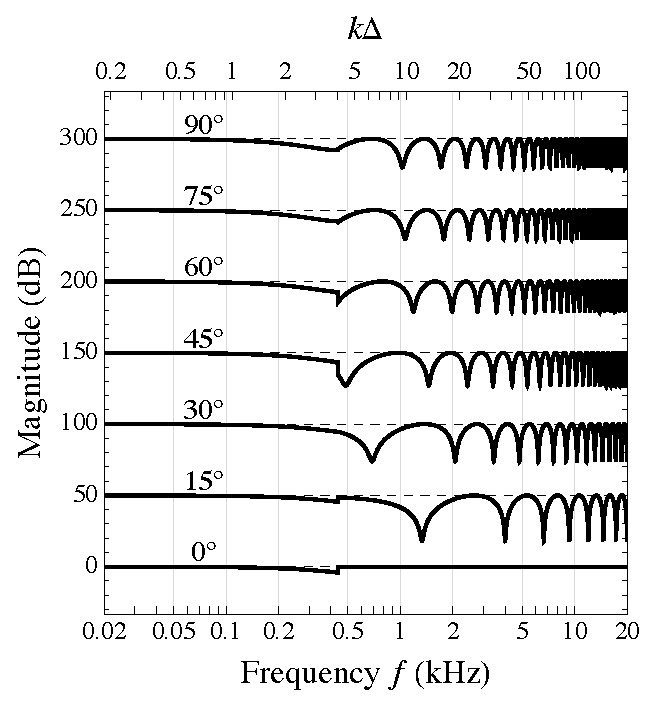
\includegraphics[width=\textwidth]{08_proposed_method/figures/sourceAz_freqResp_validhybrid.eps}
        		\caption{Hybrid filters}
        		\label{fig:08_Proposed_Method:Azimuth_Dependence:Hybrid}
    	\end{subfigure}
	
	\caption[Magnitude responses across azimuths for each interpolation filter.]{
	Magnitude responses caused by the regularized least-squares and hybrid interpolation filters for various source azimuths.
  The bottom axes show frequency in kHz while the top axes show the nondimensional frequency $k\Delta$ for a microphone spacing of $\Delta = 0.5$~m.
  For legibility, each frequency response is offset by $50$~dB and the responses have been artificially truncated (where needed) to not exceed $-45$~dB.}
	\label{fig:08_Proposed_Method:Azimuth_Dependence}
\end{figure*} %%NOTE%% vertical axis label is too complicated: |A0 / B0ref| or something

As shown in \figref{fig:08_Proposed_Method:Azimuth_Dependence:Hybrid}, the hybrid filters exhibit precisely this comb-filtering frequency response above the critical frequency, $k_0$, given in \eqnref{eq:08_Proposed_Method:Hybrid_XO_Freq}.
Below this critical frequency, however, the hybrid filter responses exhibit a wide, flat region, rather than the continued comb-filtering response exhibited by the weighted average method (as shown in \figref{fig:08_Proposed_Method:XF_CombFiltering}).
Consequently, we expect the coloration incurred by the hybrid filters to be less severe than that incurred by the weighted average method.